
% Default to the notebook output style

    


% Inherit from the specified cell style.




    
\documentclass[11pt]{article}

    
    
    \usepackage[T1]{fontenc}
    % Nicer default font (+ math font) than Computer Modern for most use cases
    \usepackage{mathpazo}

    % Basic figure setup, for now with no caption control since it's done
    % automatically by Pandoc (which extracts ![](path) syntax from Markdown).
    \usepackage{graphicx}
    % We will generate all images so they have a width \maxwidth. This means
    % that they will get their normal width if they fit onto the page, but
    % are scaled down if they would overflow the margins.
    \makeatletter
    \def\maxwidth{\ifdim\Gin@nat@width>\linewidth\linewidth
    \else\Gin@nat@width\fi}
    \makeatother
    \let\Oldincludegraphics\includegraphics
    % Set max figure width to be 80% of text width, for now hardcoded.
    \renewcommand{\includegraphics}[1]{\Oldincludegraphics[width=.8\maxwidth]{#1}}
    % Ensure that by default, figures have no caption (until we provide a
    % proper Figure object with a Caption API and a way to capture that
    % in the conversion process - todo).
    \usepackage{caption}
    \DeclareCaptionLabelFormat{nolabel}{}
    \captionsetup{labelformat=nolabel}

    \usepackage{adjustbox} % Used to constrain images to a maximum size 
    \usepackage{xcolor} % Allow colors to be defined
    \usepackage{enumerate} % Needed for markdown enumerations to work
    \usepackage{geometry} % Used to adjust the document margins
    \usepackage{amsmath} % Equations
    \usepackage{amssymb} % Equations
    \usepackage{textcomp} % defines textquotesingle
    % Hack from http://tex.stackexchange.com/a/47451/13684:
    \AtBeginDocument{%
        \def\PYZsq{\textquotesingle}% Upright quotes in Pygmentized code
    }
    \usepackage{upquote} % Upright quotes for verbatim code
    \usepackage{eurosym} % defines \euro
    \usepackage[mathletters]{ucs} % Extended unicode (utf-8) support
    \usepackage[utf8x]{inputenc} % Allow utf-8 characters in the tex document
    \usepackage{fancyvrb} % verbatim replacement that allows latex
    \usepackage{grffile} % extends the file name processing of package graphics 
                         % to support a larger range 
    % The hyperref package gives us a pdf with properly built
    % internal navigation ('pdf bookmarks' for the table of contents,
    % internal cross-reference links, web links for URLs, etc.)
    \usepackage{hyperref}
    \usepackage{longtable} % longtable support required by pandoc >1.10
    \usepackage{booktabs}  % table support for pandoc > 1.12.2
    \usepackage[inline]{enumitem} % IRkernel/repr support (it uses the enumerate* environment)
    \usepackage[normalem]{ulem} % ulem is needed to support strikethroughs (\sout)
                                % normalem makes italics be italics, not underlines
    

    
    
    % Colors for the hyperref package
    \definecolor{urlcolor}{rgb}{0,.145,.698}
    \definecolor{linkcolor}{rgb}{.71,0.21,0.01}
    \definecolor{citecolor}{rgb}{.12,.54,.11}

    % ANSI colors
    \definecolor{ansi-black}{HTML}{3E424D}
    \definecolor{ansi-black-intense}{HTML}{282C36}
    \definecolor{ansi-red}{HTML}{E75C58}
    \definecolor{ansi-red-intense}{HTML}{B22B31}
    \definecolor{ansi-green}{HTML}{00A250}
    \definecolor{ansi-green-intense}{HTML}{007427}
    \definecolor{ansi-yellow}{HTML}{DDB62B}
    \definecolor{ansi-yellow-intense}{HTML}{B27D12}
    \definecolor{ansi-blue}{HTML}{208FFB}
    \definecolor{ansi-blue-intense}{HTML}{0065CA}
    \definecolor{ansi-magenta}{HTML}{D160C4}
    \definecolor{ansi-magenta-intense}{HTML}{A03196}
    \definecolor{ansi-cyan}{HTML}{60C6C8}
    \definecolor{ansi-cyan-intense}{HTML}{258F8F}
    \definecolor{ansi-white}{HTML}{C5C1B4}
    \definecolor{ansi-white-intense}{HTML}{A1A6B2}

    % commands and environments needed by pandoc snippets
    % extracted from the output of `pandoc -s`
    \providecommand{\tightlist}{%
      \setlength{\itemsep}{0pt}\setlength{\parskip}{0pt}}
    \DefineVerbatimEnvironment{Highlighting}{Verbatim}{commandchars=\\\{\}}
    % Add ',fontsize=\small' for more characters per line
    \newenvironment{Shaded}{}{}
    \newcommand{\KeywordTok}[1]{\textcolor[rgb]{0.00,0.44,0.13}{\textbf{{#1}}}}
    \newcommand{\DataTypeTok}[1]{\textcolor[rgb]{0.56,0.13,0.00}{{#1}}}
    \newcommand{\DecValTok}[1]{\textcolor[rgb]{0.25,0.63,0.44}{{#1}}}
    \newcommand{\BaseNTok}[1]{\textcolor[rgb]{0.25,0.63,0.44}{{#1}}}
    \newcommand{\FloatTok}[1]{\textcolor[rgb]{0.25,0.63,0.44}{{#1}}}
    \newcommand{\CharTok}[1]{\textcolor[rgb]{0.25,0.44,0.63}{{#1}}}
    \newcommand{\StringTok}[1]{\textcolor[rgb]{0.25,0.44,0.63}{{#1}}}
    \newcommand{\CommentTok}[1]{\textcolor[rgb]{0.38,0.63,0.69}{\textit{{#1}}}}
    \newcommand{\OtherTok}[1]{\textcolor[rgb]{0.00,0.44,0.13}{{#1}}}
    \newcommand{\AlertTok}[1]{\textcolor[rgb]{1.00,0.00,0.00}{\textbf{{#1}}}}
    \newcommand{\FunctionTok}[1]{\textcolor[rgb]{0.02,0.16,0.49}{{#1}}}
    \newcommand{\RegionMarkerTok}[1]{{#1}}
    \newcommand{\ErrorTok}[1]{\textcolor[rgb]{1.00,0.00,0.00}{\textbf{{#1}}}}
    \newcommand{\NormalTok}[1]{{#1}}
    
    % Additional commands for more recent versions of Pandoc
    \newcommand{\ConstantTok}[1]{\textcolor[rgb]{0.53,0.00,0.00}{{#1}}}
    \newcommand{\SpecialCharTok}[1]{\textcolor[rgb]{0.25,0.44,0.63}{{#1}}}
    \newcommand{\VerbatimStringTok}[1]{\textcolor[rgb]{0.25,0.44,0.63}{{#1}}}
    \newcommand{\SpecialStringTok}[1]{\textcolor[rgb]{0.73,0.40,0.53}{{#1}}}
    \newcommand{\ImportTok}[1]{{#1}}
    \newcommand{\DocumentationTok}[1]{\textcolor[rgb]{0.73,0.13,0.13}{\textit{{#1}}}}
    \newcommand{\AnnotationTok}[1]{\textcolor[rgb]{0.38,0.63,0.69}{\textbf{\textit{{#1}}}}}
    \newcommand{\CommentVarTok}[1]{\textcolor[rgb]{0.38,0.63,0.69}{\textbf{\textit{{#1}}}}}
    \newcommand{\VariableTok}[1]{\textcolor[rgb]{0.10,0.09,0.49}{{#1}}}
    \newcommand{\ControlFlowTok}[1]{\textcolor[rgb]{0.00,0.44,0.13}{\textbf{{#1}}}}
    \newcommand{\OperatorTok}[1]{\textcolor[rgb]{0.40,0.40,0.40}{{#1}}}
    \newcommand{\BuiltInTok}[1]{{#1}}
    \newcommand{\ExtensionTok}[1]{{#1}}
    \newcommand{\PreprocessorTok}[1]{\textcolor[rgb]{0.74,0.48,0.00}{{#1}}}
    \newcommand{\AttributeTok}[1]{\textcolor[rgb]{0.49,0.56,0.16}{{#1}}}
    \newcommand{\InformationTok}[1]{\textcolor[rgb]{0.38,0.63,0.69}{\textbf{\textit{{#1}}}}}
    \newcommand{\WarningTok}[1]{\textcolor[rgb]{0.38,0.63,0.69}{\textbf{\textit{{#1}}}}}
    
    
    % Define a nice break command that doesn't care if a line doesn't already
    % exist.
    \def\br{\hspace*{\fill} \\* }
    % Math Jax compatability definitions
    \def\gt{>}
    \def\lt{<}
    % Document parameters
    \title{Assortativity and Katz vs Eigenvector Centrality}
    
    
    

    % Pygments definitions
    
\makeatletter
\def\PY@reset{\let\PY@it=\relax \let\PY@bf=\relax%
    \let\PY@ul=\relax \let\PY@tc=\relax%
    \let\PY@bc=\relax \let\PY@ff=\relax}
\def\PY@tok#1{\csname PY@tok@#1\endcsname}
\def\PY@toks#1+{\ifx\relax#1\empty\else%
    \PY@tok{#1}\expandafter\PY@toks\fi}
\def\PY@do#1{\PY@bc{\PY@tc{\PY@ul{%
    \PY@it{\PY@bf{\PY@ff{#1}}}}}}}
\def\PY#1#2{\PY@reset\PY@toks#1+\relax+\PY@do{#2}}

\expandafter\def\csname PY@tok@gd\endcsname{\def\PY@tc##1{\textcolor[rgb]{0.63,0.00,0.00}{##1}}}
\expandafter\def\csname PY@tok@gu\endcsname{\let\PY@bf=\textbf\def\PY@tc##1{\textcolor[rgb]{0.50,0.00,0.50}{##1}}}
\expandafter\def\csname PY@tok@gt\endcsname{\def\PY@tc##1{\textcolor[rgb]{0.00,0.27,0.87}{##1}}}
\expandafter\def\csname PY@tok@gs\endcsname{\let\PY@bf=\textbf}
\expandafter\def\csname PY@tok@gr\endcsname{\def\PY@tc##1{\textcolor[rgb]{1.00,0.00,0.00}{##1}}}
\expandafter\def\csname PY@tok@cm\endcsname{\let\PY@it=\textit\def\PY@tc##1{\textcolor[rgb]{0.25,0.50,0.50}{##1}}}
\expandafter\def\csname PY@tok@vg\endcsname{\def\PY@tc##1{\textcolor[rgb]{0.10,0.09,0.49}{##1}}}
\expandafter\def\csname PY@tok@vi\endcsname{\def\PY@tc##1{\textcolor[rgb]{0.10,0.09,0.49}{##1}}}
\expandafter\def\csname PY@tok@vm\endcsname{\def\PY@tc##1{\textcolor[rgb]{0.10,0.09,0.49}{##1}}}
\expandafter\def\csname PY@tok@mh\endcsname{\def\PY@tc##1{\textcolor[rgb]{0.40,0.40,0.40}{##1}}}
\expandafter\def\csname PY@tok@cs\endcsname{\let\PY@it=\textit\def\PY@tc##1{\textcolor[rgb]{0.25,0.50,0.50}{##1}}}
\expandafter\def\csname PY@tok@ge\endcsname{\let\PY@it=\textit}
\expandafter\def\csname PY@tok@vc\endcsname{\def\PY@tc##1{\textcolor[rgb]{0.10,0.09,0.49}{##1}}}
\expandafter\def\csname PY@tok@il\endcsname{\def\PY@tc##1{\textcolor[rgb]{0.40,0.40,0.40}{##1}}}
\expandafter\def\csname PY@tok@go\endcsname{\def\PY@tc##1{\textcolor[rgb]{0.53,0.53,0.53}{##1}}}
\expandafter\def\csname PY@tok@cp\endcsname{\def\PY@tc##1{\textcolor[rgb]{0.74,0.48,0.00}{##1}}}
\expandafter\def\csname PY@tok@gi\endcsname{\def\PY@tc##1{\textcolor[rgb]{0.00,0.63,0.00}{##1}}}
\expandafter\def\csname PY@tok@gh\endcsname{\let\PY@bf=\textbf\def\PY@tc##1{\textcolor[rgb]{0.00,0.00,0.50}{##1}}}
\expandafter\def\csname PY@tok@ni\endcsname{\let\PY@bf=\textbf\def\PY@tc##1{\textcolor[rgb]{0.60,0.60,0.60}{##1}}}
\expandafter\def\csname PY@tok@nl\endcsname{\def\PY@tc##1{\textcolor[rgb]{0.63,0.63,0.00}{##1}}}
\expandafter\def\csname PY@tok@nn\endcsname{\let\PY@bf=\textbf\def\PY@tc##1{\textcolor[rgb]{0.00,0.00,1.00}{##1}}}
\expandafter\def\csname PY@tok@no\endcsname{\def\PY@tc##1{\textcolor[rgb]{0.53,0.00,0.00}{##1}}}
\expandafter\def\csname PY@tok@na\endcsname{\def\PY@tc##1{\textcolor[rgb]{0.49,0.56,0.16}{##1}}}
\expandafter\def\csname PY@tok@nb\endcsname{\def\PY@tc##1{\textcolor[rgb]{0.00,0.50,0.00}{##1}}}
\expandafter\def\csname PY@tok@nc\endcsname{\let\PY@bf=\textbf\def\PY@tc##1{\textcolor[rgb]{0.00,0.00,1.00}{##1}}}
\expandafter\def\csname PY@tok@nd\endcsname{\def\PY@tc##1{\textcolor[rgb]{0.67,0.13,1.00}{##1}}}
\expandafter\def\csname PY@tok@ne\endcsname{\let\PY@bf=\textbf\def\PY@tc##1{\textcolor[rgb]{0.82,0.25,0.23}{##1}}}
\expandafter\def\csname PY@tok@nf\endcsname{\def\PY@tc##1{\textcolor[rgb]{0.00,0.00,1.00}{##1}}}
\expandafter\def\csname PY@tok@si\endcsname{\let\PY@bf=\textbf\def\PY@tc##1{\textcolor[rgb]{0.73,0.40,0.53}{##1}}}
\expandafter\def\csname PY@tok@s2\endcsname{\def\PY@tc##1{\textcolor[rgb]{0.73,0.13,0.13}{##1}}}
\expandafter\def\csname PY@tok@nt\endcsname{\let\PY@bf=\textbf\def\PY@tc##1{\textcolor[rgb]{0.00,0.50,0.00}{##1}}}
\expandafter\def\csname PY@tok@nv\endcsname{\def\PY@tc##1{\textcolor[rgb]{0.10,0.09,0.49}{##1}}}
\expandafter\def\csname PY@tok@s1\endcsname{\def\PY@tc##1{\textcolor[rgb]{0.73,0.13,0.13}{##1}}}
\expandafter\def\csname PY@tok@dl\endcsname{\def\PY@tc##1{\textcolor[rgb]{0.73,0.13,0.13}{##1}}}
\expandafter\def\csname PY@tok@ch\endcsname{\let\PY@it=\textit\def\PY@tc##1{\textcolor[rgb]{0.25,0.50,0.50}{##1}}}
\expandafter\def\csname PY@tok@m\endcsname{\def\PY@tc##1{\textcolor[rgb]{0.40,0.40,0.40}{##1}}}
\expandafter\def\csname PY@tok@gp\endcsname{\let\PY@bf=\textbf\def\PY@tc##1{\textcolor[rgb]{0.00,0.00,0.50}{##1}}}
\expandafter\def\csname PY@tok@sh\endcsname{\def\PY@tc##1{\textcolor[rgb]{0.73,0.13,0.13}{##1}}}
\expandafter\def\csname PY@tok@ow\endcsname{\let\PY@bf=\textbf\def\PY@tc##1{\textcolor[rgb]{0.67,0.13,1.00}{##1}}}
\expandafter\def\csname PY@tok@sx\endcsname{\def\PY@tc##1{\textcolor[rgb]{0.00,0.50,0.00}{##1}}}
\expandafter\def\csname PY@tok@bp\endcsname{\def\PY@tc##1{\textcolor[rgb]{0.00,0.50,0.00}{##1}}}
\expandafter\def\csname PY@tok@c1\endcsname{\let\PY@it=\textit\def\PY@tc##1{\textcolor[rgb]{0.25,0.50,0.50}{##1}}}
\expandafter\def\csname PY@tok@fm\endcsname{\def\PY@tc##1{\textcolor[rgb]{0.00,0.00,1.00}{##1}}}
\expandafter\def\csname PY@tok@o\endcsname{\def\PY@tc##1{\textcolor[rgb]{0.40,0.40,0.40}{##1}}}
\expandafter\def\csname PY@tok@kc\endcsname{\let\PY@bf=\textbf\def\PY@tc##1{\textcolor[rgb]{0.00,0.50,0.00}{##1}}}
\expandafter\def\csname PY@tok@c\endcsname{\let\PY@it=\textit\def\PY@tc##1{\textcolor[rgb]{0.25,0.50,0.50}{##1}}}
\expandafter\def\csname PY@tok@mf\endcsname{\def\PY@tc##1{\textcolor[rgb]{0.40,0.40,0.40}{##1}}}
\expandafter\def\csname PY@tok@err\endcsname{\def\PY@bc##1{\setlength{\fboxsep}{0pt}\fcolorbox[rgb]{1.00,0.00,0.00}{1,1,1}{\strut ##1}}}
\expandafter\def\csname PY@tok@mb\endcsname{\def\PY@tc##1{\textcolor[rgb]{0.40,0.40,0.40}{##1}}}
\expandafter\def\csname PY@tok@ss\endcsname{\def\PY@tc##1{\textcolor[rgb]{0.10,0.09,0.49}{##1}}}
\expandafter\def\csname PY@tok@sr\endcsname{\def\PY@tc##1{\textcolor[rgb]{0.73,0.40,0.53}{##1}}}
\expandafter\def\csname PY@tok@mo\endcsname{\def\PY@tc##1{\textcolor[rgb]{0.40,0.40,0.40}{##1}}}
\expandafter\def\csname PY@tok@kd\endcsname{\let\PY@bf=\textbf\def\PY@tc##1{\textcolor[rgb]{0.00,0.50,0.00}{##1}}}
\expandafter\def\csname PY@tok@mi\endcsname{\def\PY@tc##1{\textcolor[rgb]{0.40,0.40,0.40}{##1}}}
\expandafter\def\csname PY@tok@kn\endcsname{\let\PY@bf=\textbf\def\PY@tc##1{\textcolor[rgb]{0.00,0.50,0.00}{##1}}}
\expandafter\def\csname PY@tok@cpf\endcsname{\let\PY@it=\textit\def\PY@tc##1{\textcolor[rgb]{0.25,0.50,0.50}{##1}}}
\expandafter\def\csname PY@tok@kr\endcsname{\let\PY@bf=\textbf\def\PY@tc##1{\textcolor[rgb]{0.00,0.50,0.00}{##1}}}
\expandafter\def\csname PY@tok@s\endcsname{\def\PY@tc##1{\textcolor[rgb]{0.73,0.13,0.13}{##1}}}
\expandafter\def\csname PY@tok@kp\endcsname{\def\PY@tc##1{\textcolor[rgb]{0.00,0.50,0.00}{##1}}}
\expandafter\def\csname PY@tok@w\endcsname{\def\PY@tc##1{\textcolor[rgb]{0.73,0.73,0.73}{##1}}}
\expandafter\def\csname PY@tok@kt\endcsname{\def\PY@tc##1{\textcolor[rgb]{0.69,0.00,0.25}{##1}}}
\expandafter\def\csname PY@tok@sc\endcsname{\def\PY@tc##1{\textcolor[rgb]{0.73,0.13,0.13}{##1}}}
\expandafter\def\csname PY@tok@sb\endcsname{\def\PY@tc##1{\textcolor[rgb]{0.73,0.13,0.13}{##1}}}
\expandafter\def\csname PY@tok@sa\endcsname{\def\PY@tc##1{\textcolor[rgb]{0.73,0.13,0.13}{##1}}}
\expandafter\def\csname PY@tok@k\endcsname{\let\PY@bf=\textbf\def\PY@tc##1{\textcolor[rgb]{0.00,0.50,0.00}{##1}}}
\expandafter\def\csname PY@tok@se\endcsname{\let\PY@bf=\textbf\def\PY@tc##1{\textcolor[rgb]{0.73,0.40,0.13}{##1}}}
\expandafter\def\csname PY@tok@sd\endcsname{\let\PY@it=\textit\def\PY@tc##1{\textcolor[rgb]{0.73,0.13,0.13}{##1}}}

\def\PYZbs{\char`\\}
\def\PYZus{\char`\_}
\def\PYZob{\char`\{}
\def\PYZcb{\char`\}}
\def\PYZca{\char`\^}
\def\PYZam{\char`\&}
\def\PYZlt{\char`\<}
\def\PYZgt{\char`\>}
\def\PYZsh{\char`\#}
\def\PYZpc{\char`\%}
\def\PYZdl{\char`\$}
\def\PYZhy{\char`\-}
\def\PYZsq{\char`\'}
\def\PYZdq{\char`\"}
\def\PYZti{\char`\~}
% for compatibility with earlier versions
\def\PYZat{@}
\def\PYZlb{[}
\def\PYZrb{]}
\makeatother


    % Exact colors from NB
    \definecolor{incolor}{rgb}{0.0, 0.0, 0.5}
    \definecolor{outcolor}{rgb}{0.545, 0.0, 0.0}



    
    % Prevent overflowing lines due to hard-to-break entities
    \sloppy 
    % Setup hyperref package
    \hypersetup{
      breaklinks=true,  % so long urls are correctly broken across lines
      colorlinks=true,
      urlcolor=urlcolor,
      linkcolor=linkcolor,
      citecolor=citecolor,
      }
    % Slightly bigger margins than the latex defaults
    
    \geometry{verbose,tmargin=1in,bmargin=1in,lmargin=1in,rmargin=1in}
    
    

    \begin{document}
    
    
    \maketitle
    
    

    
    \paragraph{Purpose}\label{purpose}

We are testing the idea that all assortatively mixed graphs with
differring densities show distinct clusters in the Katz centrality vs
Eigenvector centrality plot, as shown in the figure below. More
specifically, it is supposed that in strongly assortatively mixed
graphs, the denser of the two node classes benefits more from the free
centrality in the Katz calculation than the sparser.

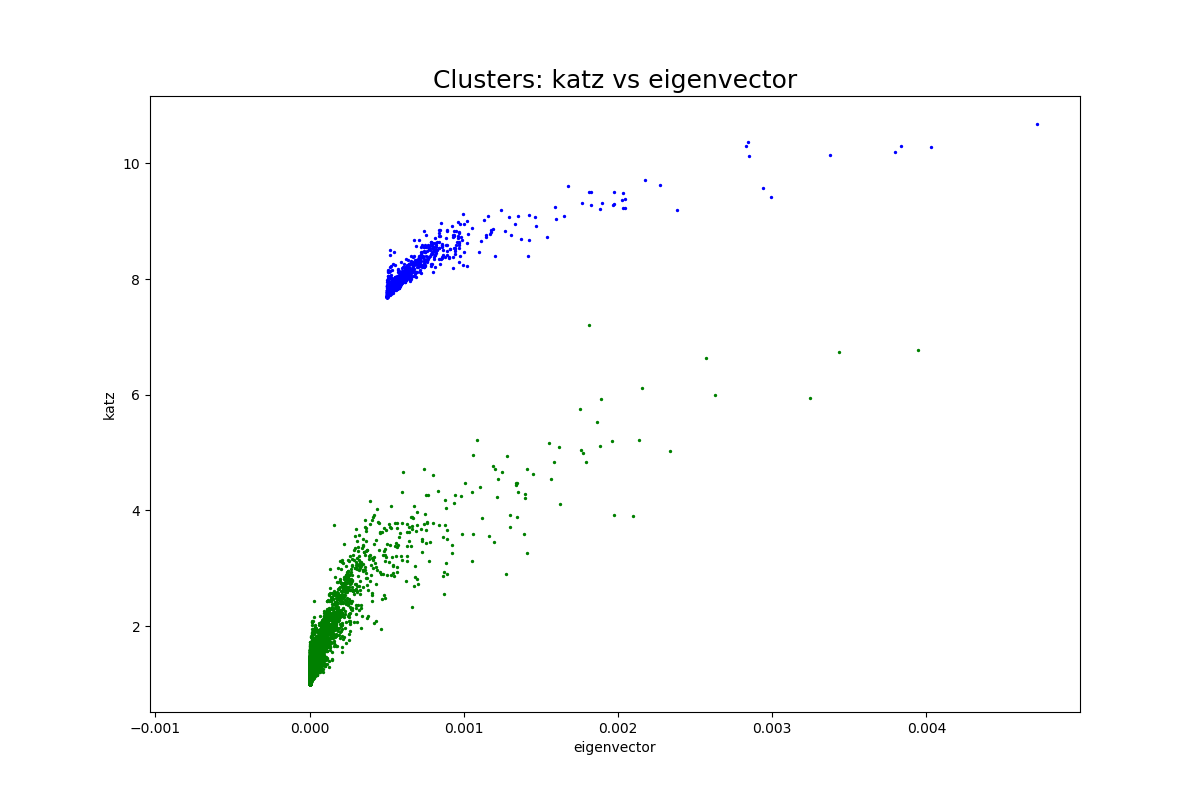
\includegraphics{katz_vs_eigenvector}

    \paragraph{Methods}\label{methods}

We will first randomly generate two graphs of different densities. These
two graphs will serve as the two node classes. A selection of nodes from
both classes will be connected to create the overall assortatively mixed
graph. Once the assortatively mixed network is created the Katz vs
eigenvector centrality plot will be generated to determine if the effect
is present.


    \begin{Verbatim}[commandchars=\\\{\}]
{\color{incolor}In [{\color{incolor}2}]:} \PY{k+kn}{import} \PY{n+nn}{zen}
        \PY{k+kn}{import} \PY{n+nn}{matplotlib.pyplot} \PY{k+kn}{as} \PY{n+nn}{plt}
        \PY{k+kn}{import} \PY{n+nn}{numpy} \PY{k+kn}{as} \PY{n+nn}{np}
\end{Verbatim}


    \begin{Verbatim}[commandchars=\\\{\}]
{\color{incolor}In [{\color{incolor}283}]:} \PY{c+c1}{\PYZsh{} first two graphs}
          \PY{n}{Size1} \PY{o}{=} \PY{l+m+mi}{1000}
          \PY{n}{Size2} \PY{o}{=} \PY{l+m+mi}{250}
          \PY{n}{Size} \PY{o}{=} \PY{n}{Size1} \PY{o}{+} \PY{n}{Size2}
          \PY{n}{G1} \PY{o}{=} \PY{n}{zen}\PY{o}{.}\PY{n}{generating}\PY{o}{.}\PY{n}{barabasi\PYZus{}albert}\PY{p}{(}\PY{n}{Size1}\PY{p}{,}\PY{l+m+mi}{2}\PY{p}{)}
          \PY{n}{G2} \PY{o}{=} \PY{n}{zen}\PY{o}{.}\PY{n}{generating}\PY{o}{.}\PY{n}{barabasi\PYZus{}albert}\PY{p}{(}\PY{n}{Size2}\PY{p}{,}\PY{l+m+mi}{30}\PY{p}{)}
          \PY{c+c1}{\PYZsh{}G1 = zen.generating.erdos\PYZus{}renyi(Size1,0.01)}
          \PY{c+c1}{\PYZsh{}G2 = zen.generating.erdos\PYZus{}renyi(Size2,0.2)}
          
          \PY{n}{gcc1} \PY{o}{=} \PY{n}{zen}\PY{o}{.}\PY{n}{algorithms}\PY{o}{.}\PY{n}{clustering}\PY{o}{.}\PY{n}{gcc}\PY{p}{(}\PY{n}{G1}\PY{p}{)}
          \PY{n}{gcc2} \PY{o}{=} \PY{n}{zen}\PY{o}{.}\PY{n}{algorithms}\PY{o}{.}\PY{n}{clustering}\PY{o}{.}\PY{n}{gcc}\PY{p}{(}\PY{n}{G2}\PY{p}{)}
          
          \PY{k}{print} \PY{l+s+s1}{\PYZsq{}}\PY{l+s+s1}{Graph 1:}\PY{l+s+s1}{\PYZsq{}}
          \PY{k}{print} \PY{l+s+s1}{\PYZsq{}}\PY{l+s+s1}{Average Degree:    }\PY{l+s+si}{\PYZpc{}.2f}\PY{l+s+s1}{\PYZsq{}}\PY{o}{\PYZpc{}}\PY{p}{(}\PY{l+m+mf}{2.0}\PY{o}{*}\PY{n}{G1}\PY{o}{.}\PY{n}{num\PYZus{}edges} \PY{o}{/}\PY{n}{G1}\PY{o}{.}\PY{n}{num\PYZus{}nodes}\PY{p}{)}
          \PY{k}{print} \PY{l+s+s1}{\PYZsq{}}\PY{l+s+s1}{Global Clustering: }\PY{l+s+si}{\PYZpc{}.3f}\PY{l+s+s1}{\PYZsq{}}\PY{o}{\PYZpc{}}\PY{k}{gcc1}
          \PY{k}{print} \PY{l+s+s1}{\PYZsq{}}\PY{l+s+s1}{\PYZsq{}}
          \PY{k}{print} \PY{l+s+s1}{\PYZsq{}}\PY{l+s+s1}{Graph 2:}\PY{l+s+s1}{\PYZsq{}}
          \PY{k}{print} \PY{l+s+s1}{\PYZsq{}}\PY{l+s+s1}{Average Degree:    }\PY{l+s+si}{\PYZpc{}.2f}\PY{l+s+s1}{\PYZsq{}}\PY{o}{\PYZpc{}}\PY{p}{(}\PY{l+m+mf}{2.0}\PY{o}{*}\PY{n}{G2}\PY{o}{.}\PY{n}{num\PYZus{}edges} \PY{o}{/}\PY{n}{G2}\PY{o}{.}\PY{n}{num\PYZus{}nodes}\PY{p}{)}
          \PY{k}{print} \PY{l+s+s1}{\PYZsq{}}\PY{l+s+s1}{Global Clustering: }\PY{l+s+si}{\PYZpc{}.3f}\PY{l+s+s1}{\PYZsq{}}\PY{o}{\PYZpc{}}\PY{k}{gcc2}
\end{Verbatim}


    \begin{Verbatim}[commandchars=\\\{\}]
Graph 1:
Average Degree:    3.99
Global Clustering: 0.008

Graph 2:
Average Degree:    52.80
Global Clustering: 0.298

    \end{Verbatim}

    \begin{Verbatim}[commandchars=\\\{\}]
{\color{incolor}In [{\color{incolor}284}]:} \PY{c+c1}{\PYZsh{} Form Overall Graph}
          \PY{n}{G} \PY{o}{=} \PY{n}{zen}\PY{o}{.}\PY{n}{Graph}\PY{p}{(}\PY{p}{)}
          \PY{k}{for} \PY{n}{i} \PY{o+ow}{in} \PY{n+nb}{range}\PY{p}{(}\PY{n}{Size}\PY{p}{)}\PY{p}{:}
              \PY{n}{G}\PY{o}{.}\PY{n}{add\PYZus{}node}\PY{p}{(}\PY{n}{i}\PY{p}{)}
          
          \PY{k}{for} \PY{n}{edge} \PY{o+ow}{in} \PY{n}{G1}\PY{o}{.}\PY{n}{edges\PYZus{}iter}\PY{p}{(}\PY{p}{)}\PY{p}{:}
              \PY{n}{u} \PY{o}{=} \PY{n}{edge}\PY{p}{[}\PY{l+m+mi}{0}\PY{p}{]}
              \PY{n}{v} \PY{o}{=} \PY{n}{edge}\PY{p}{[}\PY{l+m+mi}{1}\PY{p}{]}
              \PY{n}{G}\PY{o}{.}\PY{n}{add\PYZus{}edge}\PY{p}{(}\PY{n}{u}\PY{p}{,}\PY{n}{v}\PY{p}{)}
          
          \PY{k}{for} \PY{n}{edge} \PY{o+ow}{in} \PY{n}{G2}\PY{o}{.}\PY{n}{edges\PYZus{}iter}\PY{p}{(}\PY{p}{)}\PY{p}{:}
              \PY{n}{u} \PY{o}{=} \PY{n}{edge}\PY{p}{[}\PY{l+m+mi}{0}\PY{p}{]}\PY{o}{+}\PY{n}{Size1}
              \PY{n}{v} \PY{o}{=} \PY{n}{edge}\PY{p}{[}\PY{l+m+mi}{1}\PY{p}{]}\PY{o}{+}\PY{n}{Size1}
              \PY{n}{G}\PY{o}{.}\PY{n}{add\PYZus{}edge}\PY{p}{(}\PY{n}{u}\PY{p}{,}\PY{n}{v}\PY{p}{)}
          
          \PY{c+c1}{\PYZsh{} Select random pairs of nodes to connect the subgraphs}
          \PY{n}{EDGE\PYZus{}NUM}\PY{o}{=}\PY{l+m+mi}{400}
          \PY{n}{join\PYZus{}nodes} \PY{o}{=} \PY{n}{np}\PY{o}{.}\PY{n}{empty}\PY{p}{(}\PY{p}{(}\PY{n}{EDGE\PYZus{}NUM}\PY{p}{,}\PY{l+m+mi}{2}\PY{p}{)}\PY{p}{,}\PY{n}{dtype}\PY{o}{=}\PY{n}{np}\PY{o}{.}\PY{n}{int64}\PY{p}{)}
          \PY{n}{nodes1} \PY{o}{=} \PY{n}{np}\PY{o}{.}\PY{n}{random}\PY{o}{.}\PY{n}{randint}\PY{p}{(}\PY{l+m+mi}{0}\PY{p}{,}\PY{n}{Size1}\PY{p}{,}\PY{n}{size}\PY{o}{=}\PY{n}{EDGE\PYZus{}NUM}\PY{p}{)}
          \PY{n}{nodes2} \PY{o}{=} \PY{n}{np}\PY{o}{.}\PY{n}{random}\PY{o}{.}\PY{n}{randint}\PY{p}{(}\PY{n}{Size1}\PY{p}{,}\PY{n}{Size}\PY{p}{,}\PY{n}{size}\PY{o}{=}\PY{n}{EDGE\PYZus{}NUM}\PY{p}{)}
          \PY{n}{join\PYZus{}nodes}\PY{p}{[}\PY{p}{:}\PY{p}{,}\PY{l+m+mi}{0}\PY{p}{]} \PY{o}{=} \PY{n}{nodes1}
          \PY{n}{join\PYZus{}nodes}\PY{p}{[}\PY{p}{:}\PY{p}{,}\PY{l+m+mi}{1}\PY{p}{]} \PY{o}{=} \PY{n}{nodes2}
          
          \PY{k}{for} \PY{n}{edge} \PY{o+ow}{in} \PY{n}{join\PYZus{}nodes}\PY{p}{:}
              \PY{k}{if} \PY{o+ow}{not} \PY{n}{G}\PY{o}{.}\PY{n}{has\PYZus{}edge}\PY{p}{(}\PY{n}{edge}\PY{p}{[}\PY{l+m+mi}{0}\PY{p}{]}\PY{p}{,}\PY{n}{edge}\PY{p}{[}\PY{l+m+mi}{1}\PY{p}{]}\PY{p}{)}\PY{p}{:}
                  \PY{n}{G}\PY{o}{.}\PY{n}{add\PYZus{}edge}\PY{p}{(}\PY{n}{edge}\PY{p}{[}\PY{l+m+mi}{0}\PY{p}{]}\PY{p}{,}\PY{n}{edge}\PY{p}{[}\PY{l+m+mi}{1}\PY{p}{]}\PY{p}{)}
\end{Verbatim}


    \begin{Verbatim}[commandchars=\\\{\}]
{\color{incolor}In [{\color{incolor}285}]:} \PY{c+c1}{\PYZsh{} Modularity Calculation}
          \PY{n}{classes} \PY{o}{=} \PY{p}{\PYZob{}}\PY{l+m+mi}{0}\PY{p}{:}\PY{n}{np}\PY{o}{.}\PY{n}{arange}\PY{p}{(}\PY{l+m+mi}{0}\PY{p}{,}\PY{n}{Size1}\PY{p}{)}\PY{p}{,}\PY{l+m+mi}{1}\PY{p}{:}\PY{n}{np}\PY{o}{.}\PY{n}{arange}\PY{p}{(}\PY{n}{Size1}\PY{p}{,}\PY{n}{Size}\PY{p}{)}\PY{p}{\PYZcb{}}
          \PY{n}{Q} \PY{o}{=} \PY{n}{zen}\PY{o}{.}\PY{n}{algorithms}\PY{o}{.}\PY{n}{modularity}\PY{p}{(}\PY{n}{G}\PY{p}{,}\PY{n}{classes}\PY{p}{)}
          
          \PY{c+c1}{\PYZsh{} Maximum Modularity}
          \PY{n}{count}\PY{o}{=}\PY{l+m+mf}{0.0}
          \PY{k}{for} \PY{n}{e} \PY{o+ow}{in} \PY{n}{G}\PY{o}{.}\PY{n}{edges}\PY{p}{(}\PY{p}{)}\PY{p}{:}
              \PY{k}{if} \PY{p}{(}\PY{n}{e}\PY{p}{[}\PY{l+m+mi}{0}\PY{p}{]}\PY{o}{\PYZlt{}}\PY{n}{Size1} \PY{o+ow}{and} \PY{n}{e}\PY{p}{[}\PY{l+m+mi}{1}\PY{p}{]}\PY{o}{\PYZlt{}}\PY{n}{Size1}\PY{p}{)} \PY{o+ow}{or} \PY{p}{(}\PY{n}{e}\PY{p}{[}\PY{l+m+mi}{0}\PY{p}{]}\PY{o}{\PYZgt{}}\PY{o}{=}\PY{n}{Size1} \PY{o+ow}{and} \PY{n}{e}\PY{p}{[}\PY{l+m+mi}{1}\PY{p}{]}\PY{o}{\PYZgt{}}\PY{o}{=}\PY{n}{Size1}\PY{p}{)}\PY{p}{:}
                  \PY{n}{count} \PY{o}{+}\PY{o}{=} \PY{l+m+mi}{1}
          \PY{n}{same} \PY{o}{=} \PY{n}{count} \PY{o}{/} \PY{n}{G}\PY{o}{.}\PY{n}{num\PYZus{}edges}
          \PY{n}{rand} \PY{o}{=} \PY{n}{same} \PY{o}{\PYZhy{}} \PY{n}{Q}
          \PY{n}{qmax} \PY{o}{=} \PY{l+m+mi}{1} \PY{o}{\PYZhy{}} \PY{n}{rand}
          
          \PY{k}{print} \PY{l+s+s1}{\PYZsq{}}\PY{l+s+s1}{Modularity:      }\PY{l+s+si}{\PYZpc{}.3f}\PY{l+s+s1}{\PYZsq{}}\PY{o}{\PYZpc{}}\PY{k}{Q}
          \PY{k}{print} \PY{l+s+s1}{\PYZsq{}}\PY{l+s+s1}{Max. Modularity: }\PY{l+s+si}{\PYZpc{}.3f}\PY{l+s+s1}{\PYZsq{}}\PY{o}{\PYZpc{}}\PY{k}{qmax}
          \PY{k}{print} \PY{l+s+s1}{\PYZsq{}}\PY{l+s+s1}{Normalized Mod:  }\PY{l+s+si}{\PYZpc{}.3f}\PY{l+s+s1}{\PYZsq{}}\PY{o}{\PYZpc{}}\PY{p}{(}\PY{n}{Q}\PY{o}{/}\PY{n}{qmax}\PY{p}{)}
\end{Verbatim}


    \begin{Verbatim}[commandchars=\\\{\}]
Modularity:      0.325
Max. Modularity: 0.369
Normalized Mod:  0.880

    \end{Verbatim}

    At this point we have generated two random graphs using preferential
attachment, and joined them with 20 random edges. The resulting combined
graph is strongly assortatively mixed as indicated by the normalized
modularity value. To see if this graph indicates the same phemonenon of
boosted Katz centrality, we will display the two groups in a Katz vs
eigenvector centrality plot.

    \begin{Verbatim}[commandchars=\\\{\}]
{\color{incolor}In [{\color{incolor}286}]:} \PY{k}{def} \PY{n+nf}{katz}\PY{p}{(}\PY{n}{G}\PY{p}{,}\PY{n}{tol}\PY{o}{=}\PY{l+m+mf}{0.01}\PY{p}{,}\PY{n}{max\PYZus{}iter}\PY{o}{=}\PY{l+m+mi}{1000}\PY{p}{,}\PY{n}{alpha}\PY{o}{=}\PY{l+m+mf}{0.001}\PY{p}{,}\PY{n}{beta}\PY{o}{=}\PY{l+m+mi}{1}\PY{p}{)}\PY{p}{:}
              \PY{n}{iteration} \PY{o}{=} \PY{l+m+mi}{0}
              \PY{n}{centrality} \PY{o}{=} \PY{n}{np}\PY{o}{.}\PY{n}{zeros}\PY{p}{(}\PY{n}{G}\PY{o}{.}\PY{n}{num\PYZus{}nodes}\PY{p}{)}
              \PY{k}{while} \PY{n}{iteration} \PY{o}{\PYZlt{}} \PY{n}{max\PYZus{}iter}\PY{p}{:}
                  \PY{n}{iteration} \PY{o}{+}\PY{o}{=} \PY{l+m+mi}{1}          \PY{c+c1}{\PYZsh{} increment iteration count}
                  \PY{n}{centrality\PYZus{}old} \PY{o}{=} \PY{n}{centrality}\PY{o}{.}\PY{n}{copy}\PY{p}{(}\PY{p}{)}
          
                  \PY{k}{for} \PY{n}{node} \PY{o+ow}{in} \PY{n}{G}\PY{o}{.}\PY{n}{nodes\PYZus{}}\PY{p}{(}\PY{p}{)}\PY{p}{:}
                      \PY{n}{Ax} \PY{o}{=} \PY{l+m+mi}{0}
                      \PY{k}{for} \PY{n}{neighbor} \PY{o+ow}{in} \PY{n}{G}\PY{o}{.}\PY{n}{neighbors\PYZus{}}\PY{p}{(}\PY{n}{node}\PY{p}{)}\PY{p}{:}
                          \PY{c+c1}{\PYZsh{}weight = G.weight\PYZus{}(G.edge\PYZus{}idx\PYZus{}(neighbor,node))}
                          \PY{c+c1}{\PYZsh{}Ax += np.multiply(centrality[neighbor],weight)}
          
                          \PY{n}{Ax} \PY{o}{+}\PY{o}{=} \PY{n}{centrality}\PY{p}{[}\PY{n}{neighbor}\PY{p}{]}      \PY{c+c1}{\PYZsh{}exclude weight due to overflow in multiplication}
          
                      \PY{n}{centrality}\PY{p}{[}\PY{n}{node}\PY{p}{]} \PY{o}{=} \PY{n}{np}\PY{o}{.}\PY{n}{multiply}\PY{p}{(}\PY{n}{alpha}\PY{p}{,}\PY{n}{Ax}\PY{p}{)}\PY{o}{+}\PY{n}{beta}
          
                  \PY{k}{if} \PY{n}{np}\PY{o}{.}\PY{n}{sum}\PY{p}{(}\PY{n}{np}\PY{o}{.}\PY{n}{abs}\PY{p}{(}\PY{n}{np}\PY{o}{.}\PY{n}{subtract}\PY{p}{(}\PY{n}{centrality}\PY{p}{,}\PY{n}{centrality\PYZus{}old}\PY{p}{)}\PY{p}{)}\PY{p}{)} \PY{o}{\PYZlt{}} \PY{n}{tol}\PY{p}{:}
                      \PY{k}{return} \PY{n}{centrality}
          
          \PY{n}{evc} \PY{o}{=} \PY{n}{zen}\PY{o}{.}\PY{n}{algorithms}\PY{o}{.}\PY{n}{eigenvector\PYZus{}centrality\PYZus{}}\PY{p}{(}\PY{n}{G}\PY{p}{)}
          \PY{n}{kc} \PY{o}{=} \PY{n}{katz}\PY{p}{(}\PY{n}{G}\PY{p}{)}
          \PY{n}{plt}\PY{o}{.}\PY{n}{scatter}\PY{p}{(}\PY{n}{evc}\PY{p}{[}\PY{p}{:}\PY{n}{Size1}\PY{p}{]}\PY{p}{,}\PY{n}{kc}\PY{p}{[}\PY{p}{:}\PY{n}{Size1}\PY{p}{]}\PY{p}{,}\PY{n}{c}\PY{o}{=}\PY{l+s+s1}{\PYZsq{}}\PY{l+s+s1}{g}\PY{l+s+s1}{\PYZsq{}}\PY{p}{,}\PY{n}{s}\PY{o}{=}\PY{l+m+mi}{2}\PY{p}{,}\PY{n}{label}\PY{o}{=}\PY{l+s+s1}{\PYZsq{}}\PY{l+s+s1}{Sparse Subgraph}\PY{l+s+s1}{\PYZsq{}}\PY{p}{)}
          \PY{n}{plt}\PY{o}{.}\PY{n}{scatter}\PY{p}{(}\PY{n}{evc}\PY{p}{[}\PY{n}{Size1}\PY{p}{:}\PY{p}{]}\PY{p}{,}\PY{n}{kc}\PY{p}{[}\PY{n}{Size1}\PY{p}{:}\PY{p}{]}\PY{p}{,}\PY{n}{c}\PY{o}{=}\PY{l+s+s1}{\PYZsq{}}\PY{l+s+s1}{b}\PY{l+s+s1}{\PYZsq{}}\PY{p}{,}\PY{n}{s}\PY{o}{=}\PY{l+m+mi}{2}\PY{p}{,}\PY{n}{label}\PY{o}{=}\PY{l+s+s1}{\PYZsq{}}\PY{l+s+s1}{Dense Subgraph}\PY{l+s+s1}{\PYZsq{}}\PY{p}{)}
          \PY{n}{plt}\PY{o}{.}\PY{n}{xlabel}\PY{p}{(}\PY{l+s+s1}{\PYZsq{}}\PY{l+s+s1}{Eigenvector Centrality}\PY{l+s+s1}{\PYZsq{}}\PY{p}{)}
          \PY{n}{plt}\PY{o}{.}\PY{n}{ylabel}\PY{p}{(}\PY{l+s+s1}{\PYZsq{}}\PY{l+s+s1}{Katz Centrality}\PY{l+s+s1}{\PYZsq{}}\PY{p}{)}
          \PY{n}{plt}\PY{o}{.}\PY{n}{legend}\PY{p}{(}\PY{p}{)}
          \PY{n}{plt}\PY{o}{.}\PY{n}{show}\PY{p}{(}\PY{p}{)}
\end{Verbatim}


    \begin{center}
    \adjustimage{max size={0.9\linewidth}{0.9\paperheight}}{output_8_0.png}
    \end{center}
    { \hspace*{\fill} \\}
    
    This resulting plot clearly shows distinct behavior in the two classes
of nodes. A linear regression of each class's plot will yeild different
slopes. But the separation of the classes in this resulting plot is
different from the initial plot. The initial plot showed a scaled and
translation relationship between the classes. This resulting plot shows
a scaled and rotation relationship.

Interestingly, however, the plot of eigenvector vs katz centrality more
closely resembles the initial plot.

    \begin{Verbatim}[commandchars=\\\{\}]
{\color{incolor}In [{\color{incolor}287}]:} \PY{n}{plt}\PY{o}{.}\PY{n}{scatter}\PY{p}{(}\PY{n}{kc}\PY{p}{[}\PY{p}{:}\PY{n}{Size1}\PY{p}{]}\PY{p}{,}\PY{n}{evc}\PY{p}{[}\PY{p}{:}\PY{n}{Size1}\PY{p}{]}\PY{p}{,}\PY{n}{c}\PY{o}{=}\PY{l+s+s1}{\PYZsq{}}\PY{l+s+s1}{g}\PY{l+s+s1}{\PYZsq{}}\PY{p}{,}\PY{n}{s}\PY{o}{=}\PY{l+m+mi}{2}\PY{p}{,}\PY{n}{label}\PY{o}{=}\PY{l+s+s1}{\PYZsq{}}\PY{l+s+s1}{Sparse Subgraph}\PY{l+s+s1}{\PYZsq{}}\PY{p}{)}
          \PY{n}{plt}\PY{o}{.}\PY{n}{scatter}\PY{p}{(}\PY{n}{kc}\PY{p}{[}\PY{n}{Size1}\PY{p}{:}\PY{p}{]}\PY{p}{,}\PY{n}{evc}\PY{p}{[}\PY{n}{Size1}\PY{p}{:}\PY{p}{]}\PY{p}{,}\PY{n}{c}\PY{o}{=}\PY{l+s+s1}{\PYZsq{}}\PY{l+s+s1}{b}\PY{l+s+s1}{\PYZsq{}}\PY{p}{,}\PY{n}{s}\PY{o}{=}\PY{l+m+mi}{2}\PY{p}{,}\PY{n}{label}\PY{o}{=}\PY{l+s+s1}{\PYZsq{}}\PY{l+s+s1}{Dense Subgraph}\PY{l+s+s1}{\PYZsq{}}\PY{p}{)}
          \PY{n}{plt}\PY{o}{.}\PY{n}{ylabel}\PY{p}{(}\PY{l+s+s1}{\PYZsq{}}\PY{l+s+s1}{Eigenvector Centrality}\PY{l+s+s1}{\PYZsq{}}\PY{p}{)}
          \PY{n}{plt}\PY{o}{.}\PY{n}{xlabel}\PY{p}{(}\PY{l+s+s1}{\PYZsq{}}\PY{l+s+s1}{Katz Centrality}\PY{l+s+s1}{\PYZsq{}}\PY{p}{)}
          \PY{n}{plt}\PY{o}{.}\PY{n}{legend}\PY{p}{(}\PY{p}{)}
          \PY{n}{plt}\PY{o}{.}\PY{n}{show}\PY{p}{(}\PY{p}{)}
\end{Verbatim}


    \begin{center}
    \adjustimage{max size={0.9\linewidth}{0.9\paperheight}}{output_10_0.png}
    \end{center}
    { \hspace*{\fill} \\}
    
    It is unlikely that a mistake was made in the axis labeling in the
initial plot, since the scale of the axis match with what is expected.
Eigenvector centralities are typically much less than 1, where as Katz
centralities are bounded below by \(\beta\) (set to 1 in this case).

    \begin{center}\rule{0.5\linewidth}{\linethickness}\end{center}

Now looking at a real world network with pre-labeled communities. The
\href{https://snap.stanford.edu/data/email-Eu-core.html}{Eu-core
network} is an email network that "contains 'ground-truth' community
memberships of the nodes. Each individual belongs to exactly one of 42
departments at the research institute". Plotting katz centrality against
eigenvector centrality for each department may show the clustering
phenomenon seen above.

    \begin{Verbatim}[commandchars=\\\{\}]
{\color{incolor}In [{\color{incolor}145}]:} \PY{k+kn}{import} \PY{n+nn}{pandas} \PY{k+kn}{as} \PY{n+nn}{pd}
          \PY{n}{Department} \PY{o}{=} \PY{n}{pd}\PY{o}{.}\PY{n}{read\PYZus{}csv}\PY{p}{(}\PY{l+s+s1}{\PYZsq{}}\PY{l+s+s1}{email\PYZhy{}Eu\PYZhy{}core\PYZhy{}department\PYZhy{}labels.txt}\PY{l+s+s1}{\PYZsq{}}\PY{p}{,}\PY{n}{delimiter}\PY{o}{=}\PY{l+s+s1}{\PYZsq{}}\PY{l+s+s1}{ }\PY{l+s+s1}{\PYZsq{}}\PY{p}{,}\PYZbs{}
                                   \PY{n}{header}\PY{o}{=}\PY{n+nb+bp}{None}\PY{p}{,}\PY{n}{names}\PY{o}{=}\PY{p}{[}\PY{l+s+s1}{\PYZsq{}}\PY{l+s+s1}{Node}\PY{l+s+s1}{\PYZsq{}}\PY{p}{,}\PY{l+s+s1}{\PYZsq{}}\PY{l+s+s1}{Department}\PY{l+s+s1}{\PYZsq{}}\PY{p}{]}\PY{p}{)}
          
          \PY{n}{departmentGroupings} \PY{o}{=} \PY{n}{Department}\PY{o}{.}\PY{n}{groupby}\PY{p}{(}\PY{l+s+s1}{\PYZsq{}}\PY{l+s+s1}{Department}\PY{l+s+s1}{\PYZsq{}}\PY{p}{)}\PY{o}{.}\PY{n}{apply}\PY{p}{(}\PY{k}{lambda} \PY{n}{x}\PY{p}{:} \PY{n}{x}\PY{p}{[}\PY{l+s+s1}{\PYZsq{}}\PY{l+s+s1}{Node}\PY{l+s+s1}{\PYZsq{}}\PY{p}{]}\PY{p}{)}
          
          \PY{n}{Communities} \PY{o}{=} \PY{p}{\PYZob{}}\PY{p}{\PYZcb{}}
          \PY{k}{for} \PY{n}{dept} \PY{o+ow}{in} \PY{n}{departmentGroupings}\PY{o}{.}\PY{n}{index}\PY{o}{.}\PY{n}{get\PYZus{}level\PYZus{}values}\PY{p}{(}\PY{l+m+mi}{0}\PY{p}{)}\PY{o}{.}\PY{n}{unique}\PY{p}{(}\PY{p}{)}\PY{p}{:}
              \PY{n}{Communities}\PY{p}{[}\PY{n}{dept}\PY{p}{]} \PY{o}{=} \PY{n}{departmentGroupings}\PY{o}{.}\PY{n}{loc}\PY{p}{[}\PY{n}{dept}\PY{p}{]}\PY{o}{.}\PY{n}{values}\PY{o}{.}\PY{n}{astype}\PY{p}{(}\PY{n+nb}{str}\PY{p}{)}
          \PY{n}{Department}\PY{o}{.}\PY{n}{set\PYZus{}index}\PY{p}{(}\PY{l+s+s1}{\PYZsq{}}\PY{l+s+s1}{Node}\PY{l+s+s1}{\PYZsq{}}\PY{p}{,}\PY{n}{inplace}\PY{o}{=}\PY{n+nb+bp}{True}\PY{p}{)}
\end{Verbatim}


    \begin{Verbatim}[commandchars=\\\{\}]
{\color{incolor}In [{\color{incolor}130}]:} \PY{n}{G\PYZus{}eu\PYZus{}email} \PY{o}{=} \PY{n}{zen}\PY{o}{.}\PY{n}{io}\PY{o}{.}\PY{n}{edgelist}\PY{o}{.}\PY{n}{read}\PY{p}{(}\PY{l+s+s1}{\PYZsq{}}\PY{l+s+s1}{email\PYZhy{}Eu\PYZhy{}core.txt}\PY{l+s+s1}{\PYZsq{}}\PY{p}{,}\PY{n}{directed}\PY{o}{=}\PY{n+nb+bp}{True}\PY{p}{)} \PY{c+c1}{\PYZsh{} as undirected showed similar results.}
          
          \PY{n}{evc} \PY{o}{=} \PY{n}{zen}\PY{o}{.}\PY{n}{centrality}\PY{o}{.}\PY{n}{eigenvector\PYZus{}centrality\PYZus{}}\PY{p}{(}\PY{n}{G\PYZus{}eu\PYZus{}email}\PY{p}{)}
          \PY{n}{kc} \PY{o}{=} \PY{n}{katz}\PY{p}{(}\PY{n}{G\PYZus{}eu\PYZus{}email}\PY{p}{)}
\end{Verbatim}


    \begin{Verbatim}[commandchars=\\\{\}]
{\color{incolor}In [{\color{incolor}137}]:} \PY{n}{depts} \PY{o}{=} \PY{n}{Department}\PY{p}{[}\PY{l+s+s1}{\PYZsq{}}\PY{l+s+s1}{Department}\PY{l+s+s1}{\PYZsq{}}\PY{p}{]}\PY{o}{.}\PY{n}{unique}\PY{p}{(}\PY{p}{)}
          \PY{n}{depts}\PY{o}{.}\PY{n}{sort}\PY{p}{(}\PY{p}{)}
          \PY{n}{fig} \PY{o}{=} \PY{n}{plt}\PY{o}{.}\PY{n}{figure}\PY{p}{(}\PY{n}{figsize}\PY{o}{=}\PY{p}{(}\PY{l+m+mi}{12}\PY{p}{,}\PY{l+m+mi}{8}\PY{p}{)}\PY{p}{)}
          \PY{k}{for} \PY{n}{dept} \PY{o+ow}{in} \PY{n}{depts}\PY{p}{:}
              \PY{n}{nodes} \PY{o}{=} \PY{n}{Department}\PY{p}{[}\PY{n}{Department}\PY{p}{[}\PY{l+s+s1}{\PYZsq{}}\PY{l+s+s1}{Department}\PY{l+s+s1}{\PYZsq{}}\PY{p}{]}\PY{o}{==}\PY{n}{dept}\PY{p}{]}\PY{o}{.}\PY{n}{index}\PY{o}{.}\PY{n}{values}\PY{o}{.}\PY{n}{tolist}\PY{p}{(}\PY{p}{)}
              \PY{n}{plt}\PY{o}{.}\PY{n}{scatter}\PY{p}{(}\PY{n}{evc}\PY{p}{[}\PY{n}{nodes}\PY{p}{]}\PY{p}{,}\PY{n}{kc}\PY{p}{[}\PY{n}{nodes}\PY{p}{]}\PY{p}{,}\PY{n}{s}\PY{o}{=}\PY{l+m+mi}{2}\PY{p}{,}\PY{n}{label}\PY{o}{=}\PY{l+s+s1}{\PYZsq{}}\PY{l+s+s1}{Dept. }\PY{l+s+si}{\PYZpc{}d}\PY{l+s+s1}{\PYZsq{}}\PY{o}{\PYZpc{}}\PY{k}{dept})
          \PY{n}{plt}\PY{o}{.}\PY{n}{legend}\PY{p}{(}\PY{n}{ncol}\PY{o}{=}\PY{l+m+mi}{2}\PY{p}{)}
          \PY{c+c1}{\PYZsh{}plt.gca().set\PYZus{}xscale(\PYZsq{}log\PYZsq{})}
          \PY{c+c1}{\PYZsh{}plt.gca().set\PYZus{}yscale(\PYZsq{}log\PYZsq{})}
          \PY{n}{plt}\PY{o}{.}\PY{n}{xlabel}\PY{p}{(}\PY{l+s+s1}{\PYZsq{}}\PY{l+s+s1}{Eigenvector Centrality}\PY{l+s+s1}{\PYZsq{}}\PY{p}{)}
          \PY{n}{plt}\PY{o}{.}\PY{n}{ylabel}\PY{p}{(}\PY{l+s+s1}{\PYZsq{}}\PY{l+s+s1}{Katz Centrality}\PY{l+s+s1}{\PYZsq{}}\PY{p}{)}
          \PY{n}{plt}\PY{o}{.}\PY{n}{show}\PY{p}{(}\PY{p}{)}
\end{Verbatim}


    \begin{center}
    \adjustimage{max size={0.9\linewidth}{0.9\paperheight}}{output_15_0.png}
    \end{center}
    { \hspace*{\fill} \\}
    
    Here there is not a lot of distinguishability between the different
departments. All nodes tend to fall in the same overall trend. This may
be because the network is not strongly assortatively mixed

    \begin{Verbatim}[commandchars=\\\{\}]
{\color{incolor}In [{\color{incolor}155}]:} \PY{n}{G\PYZus{}eu\PYZus{}skel} \PY{o}{=} \PY{n}{G\PYZus{}eu\PYZus{}email}\PY{o}{.}\PY{n}{skeleton}\PY{p}{(}\PY{p}{)}
          
          \PY{n}{Q} \PY{o}{=} \PY{n}{zen}\PY{o}{.}\PY{n}{algorithms}\PY{o}{.}\PY{n}{modularity}\PY{p}{(}\PY{n}{G\PYZus{}eu\PYZus{}skel}\PY{p}{,}\PY{n}{Communities}\PY{p}{)}
          
          \PY{c+c1}{\PYZsh{} Maximum Modularity}
          \PY{n}{count}\PY{o}{=}\PY{l+m+mf}{0.0}
          \PY{k}{for} \PY{n}{e} \PY{o+ow}{in} \PY{n}{G\PYZus{}eu\PYZus{}skel}\PY{o}{.}\PY{n}{edges}\PY{p}{(}\PY{p}{)}\PY{p}{:}
              \PY{k}{if} \PY{n}{Department}\PY{o}{.}\PY{n}{loc}\PY{p}{[}\PY{n+nb}{int}\PY{p}{(}\PY{n}{e}\PY{p}{[}\PY{l+m+mi}{0}\PY{p}{]}\PY{p}{)}\PY{p}{,}\PY{l+s+s1}{\PYZsq{}}\PY{l+s+s1}{Department}\PY{l+s+s1}{\PYZsq{}}\PY{p}{]} \PY{o}{==} \PY{n}{Department}\PY{o}{.}\PY{n}{loc}\PY{p}{[}\PY{n+nb}{int}\PY{p}{(}\PY{n}{e}\PY{p}{[}\PY{l+m+mi}{1}\PY{p}{]}\PY{p}{)}\PY{p}{,}\PY{l+s+s1}{\PYZsq{}}\PY{l+s+s1}{Department}\PY{l+s+s1}{\PYZsq{}}\PY{p}{]}\PY{p}{:}
                  \PY{n}{count} \PY{o}{+}\PY{o}{=} \PY{l+m+mi}{1}
          \PY{n}{same} \PY{o}{=} \PY{n}{count} \PY{o}{/} \PY{n}{G\PYZus{}eu\PYZus{}skel}\PY{o}{.}\PY{n}{num\PYZus{}edges}
          \PY{n}{rand} \PY{o}{=} \PY{n}{same} \PY{o}{\PYZhy{}} \PY{n}{Q}
          \PY{n}{qmax} \PY{o}{=} \PY{l+m+mi}{1} \PY{o}{\PYZhy{}} \PY{n}{rand}
          
          \PY{k}{print} \PY{l+s+s1}{\PYZsq{}}\PY{l+s+s1}{Modularity:      }\PY{l+s+si}{\PYZpc{}.3f}\PY{l+s+s1}{\PYZsq{}}\PY{o}{\PYZpc{}}\PY{k}{Q}
          \PY{k}{print} \PY{l+s+s1}{\PYZsq{}}\PY{l+s+s1}{Max. Modularity: }\PY{l+s+si}{\PYZpc{}.3f}\PY{l+s+s1}{\PYZsq{}}\PY{o}{\PYZpc{}}\PY{k}{qmax}
          \PY{k}{print} \PY{l+s+s1}{\PYZsq{}}\PY{l+s+s1}{Normalized Mod:  }\PY{l+s+si}{\PYZpc{}.3f}\PY{l+s+s1}{\PYZsq{}}\PY{o}{\PYZpc{}}\PY{p}{(}\PY{n}{Q}\PY{o}{/}\PY{n}{qmax}\PY{p}{)}
\end{Verbatim}


    \begin{Verbatim}[commandchars=\\\{\}]
Modularity:      0.314
Max. Modularity: 0.953
Normalized Mod:  0.329

    \end{Verbatim}

    The preivous networks that demonstrated the distinct clusters in the
Katz vs eigenvector centrality had normalized nodularity values closer
to 1 than is seen in the Eu-core network.

\begin{center}\rule{0.5\linewidth}{\linethickness}\end{center}

Let's take another larger network from SNAP with pre-determined
communities, looking only at the subgraph of nodes belonging to the two
largest communities.
"\href{https://snap.stanford.edu/data/com-DBLP.html}{The DBLP computer
science bibliography} provides a comprehensive list of research papers
in computer science. We construct a co-authorship network where two
authors are connected if they publish at least one paper together."

    \begin{Verbatim}[commandchars=\\\{\}]
{\color{incolor}In [{\color{incolor}162}]:} \PY{n}{dblp\PYZus{}df} \PY{o}{=} \PY{n}{pd}\PY{o}{.}\PY{n}{DataFrame}\PY{p}{(}\PY{n}{columns}\PY{o}{=}\PY{p}{[}\PY{l+s+s1}{\PYZsq{}}\PY{l+s+s1}{Node}\PY{l+s+s1}{\PYZsq{}}\PY{p}{,}\PY{l+s+s1}{\PYZsq{}}\PY{l+s+s1}{Community}\PY{l+s+s1}{\PYZsq{}}\PY{p}{]}\PY{p}{)}
          
          \PY{n}{idx}\PY{o}{=}\PY{l+m+mi}{0}
          \PY{n}{comm}\PY{o}{=}\PY{l+m+mi}{0}
          \PY{k}{for} \PY{n}{line} \PY{o+ow}{in} \PY{n}{log\PYZus{}progress}\PY{p}{(}\PY{n+nb}{open}\PY{p}{(}\PY{l+s+s1}{\PYZsq{}}\PY{l+s+s1}{com\PYZhy{}dblp.top5000.cmty.txt}\PY{l+s+s1}{\PYZsq{}}\PY{p}{)}\PY{p}{,}\PY{n}{every}\PY{o}{=}\PY{l+m+mi}{1}\PY{p}{,}\PY{n}{size}\PY{o}{=}\PY{l+m+mi}{5000}\PY{p}{)}\PY{p}{:}
              \PY{n}{nodes} \PY{o}{=} \PY{n}{line}\PY{o}{.}\PY{n}{split}\PY{p}{(}\PY{l+s+s1}{\PYZsq{}}\PY{l+s+se}{\PYZbs{}t}\PY{l+s+s1}{\PYZsq{}}\PY{p}{)}
              \PY{k}{for} \PY{n}{node} \PY{o+ow}{in} \PY{n}{nodes}\PY{p}{:}
                  \PY{n}{dblp\PYZus{}df}\PY{o}{.}\PY{n}{loc}\PY{p}{[}\PY{n}{idx}\PY{p}{]} \PY{o}{=} \PY{p}{[}\PY{n+nb}{int}\PY{p}{(}\PY{n}{node}\PY{p}{)}\PY{p}{,} \PY{n}{comm}\PY{p}{]}
                  \PY{n}{idx}\PY{o}{+}\PY{o}{=}\PY{l+m+mi}{1}
              \PY{n}{comm}\PY{o}{+}\PY{o}{=}\PY{l+m+mi}{1}
          
          \PY{n}{dblp\PYZus{}df}\PY{o}{.}\PY{n}{head}\PY{p}{(}\PY{p}{)}
\end{Verbatim}


    
    \begin{verbatim}
VBox(children=(HTML(value=u''), IntProgress(value=0, max=5000)))
    \end{verbatim}

    
\begin{Verbatim}[commandchars=\\\{\}]
{\color{outcolor}Out[{\color{outcolor}162}]:}      Node Community
          0  105653         0
          1  105654         0
          2  210737         0
          3  210738         0
          4  210739         0
\end{Verbatim}
            
    \begin{Verbatim}[commandchars=\\\{\}]
{\color{incolor}In [{\color{incolor}180}]:} \PY{n}{TwoLargestCom} \PY{o}{=} \PY{n}{dblp\PYZus{}df}\PY{o}{.}\PY{n}{groupby}\PY{p}{(}\PY{l+s+s1}{\PYZsq{}}\PY{l+s+s1}{Community}\PY{l+s+s1}{\PYZsq{}}\PY{p}{)}\PY{o}{.}\PY{n}{count}\PY{p}{(}\PY{p}{)}\PY{o}{.}\PY{n}{sort\PYZus{}values}\PY{p}{(}\PY{l+s+s1}{\PYZsq{}}\PY{l+s+s1}{Node}\PY{l+s+s1}{\PYZsq{}}\PY{p}{,}\PY{n}{ascending}\PY{o}{=}\PY{n+nb+bp}{False}\PY{p}{)}\PY{o}{.}\PY{n}{iloc}\PY{p}{[}\PY{p}{:}\PY{l+m+mi}{2}\PY{p}{]}\PY{o}{.}\PY{n}{index}\PY{o}{.}\PY{n}{values}
          
          \PY{n}{sampled\PYZus{}nodes}\PY{o}{=}\PY{n}{dblp\PYZus{}df}\PY{p}{[}\PY{p}{(}\PY{n}{dblp\PYZus{}df}\PY{p}{[}\PY{l+s+s1}{\PYZsq{}}\PY{l+s+s1}{Community}\PY{l+s+s1}{\PYZsq{}}\PY{p}{]}\PY{o}{==}\PY{n}{TwoLargestCom}\PY{p}{[}\PY{l+m+mi}{0}\PY{p}{]}\PY{p}{)}\PY{o}{|}\PYZbs{}
                                \PY{p}{(}\PY{n}{dblp\PYZus{}df}\PY{p}{[}\PY{l+s+s1}{\PYZsq{}}\PY{l+s+s1}{Community}\PY{l+s+s1}{\PYZsq{}}\PY{p}{]}\PY{o}{==}\PY{n}{TwoLargestCom}\PY{p}{[}\PY{l+m+mi}{1}\PY{p}{]}\PY{p}{)}\PY{p}{]}\PY{o}{.}\PY{n}{set\PYZus{}index}\PY{p}{(}\PY{l+s+s1}{\PYZsq{}}\PY{l+s+s1}{Node}\PY{l+s+s1}{\PYZsq{}}\PY{p}{)}
\end{Verbatim}


    \begin{Verbatim}[commandchars=\\\{\}]
{\color{incolor}In [{\color{incolor}224}]:} \PY{n}{G} \PY{o}{=} \PY{n}{zen}\PY{o}{.}\PY{n}{Graph}\PY{p}{(}\PY{p}{)}
          \PY{k}{for} \PY{n}{line} \PY{o+ow}{in} \PY{n}{log\PYZus{}progress}\PY{p}{(}\PY{n+nb}{open}\PY{p}{(}\PY{l+s+s1}{\PYZsq{}}\PY{l+s+s1}{com\PYZhy{}dblp.ungraph.txt}\PY{l+s+s1}{\PYZsq{}}\PY{p}{)}\PY{p}{,}\PY{n}{every}\PY{o}{=}\PY{l+m+mi}{1}\PY{p}{,}\PY{n}{size}\PY{o}{=}\PY{l+m+mi}{1049870}\PY{p}{)}\PY{p}{:}
              \PY{n}{info} \PY{o}{=} \PY{n}{line}\PY{o}{.}\PY{n}{split}\PY{p}{(}\PY{l+s+s1}{\PYZsq{}}\PY{l+s+se}{\PYZbs{}t}\PY{l+s+s1}{\PYZsq{}}\PY{p}{)}
              \PY{n}{n1} \PY{o}{=} \PY{n+nb}{int}\PY{p}{(}\PY{n}{info}\PY{p}{[}\PY{l+m+mi}{0}\PY{p}{]}\PY{p}{)}
              \PY{n}{n2} \PY{o}{=} \PY{n+nb}{int}\PY{p}{(}\PY{n}{info}\PY{p}{[}\PY{l+m+mi}{1}\PY{p}{]}\PY{p}{)}
              
              \PY{n}{node1\PYZus{}in} \PY{o}{=} \PY{n+nb+bp}{True}
              \PY{k}{try}\PY{p}{:}
                  \PY{n}{\PYZus{}} \PY{o}{=} \PY{n}{sampled\PYZus{}nodes}\PY{o}{.}\PY{n}{loc}\PY{p}{[}\PY{n}{n1}\PY{p}{,}\PY{p}{:}\PY{p}{]}
              \PY{k}{except} \PY{n+ne}{KeyError}\PY{p}{:}
                  \PY{c+c1}{\PYZsh{} not in comm}
                  \PY{n}{node1\PYZus{}in} \PY{o}{=} \PY{n+nb+bp}{False}
                  
              \PY{n}{node2\PYZus{}in} \PY{o}{=} \PY{n+nb+bp}{True}
              \PY{k}{try}\PY{p}{:}
                  \PY{n}{\PYZus{}} \PY{o}{=} \PY{n}{sampled\PYZus{}nodes}\PY{o}{.}\PY{n}{loc}\PY{p}{[}\PY{n}{n2}\PY{p}{,}\PY{p}{:}\PY{p}{]}
              \PY{k}{except} \PY{n+ne}{KeyError}\PY{p}{:}
                  \PY{c+c1}{\PYZsh{} not in comm}
                  \PY{n}{node2\PYZus{}in} \PY{o}{=} \PY{n+nb+bp}{False}
              
              \PY{k}{if} \PY{n}{node1\PYZus{}in} \PY{o+ow}{and} \PY{n}{node2\PYZus{}in}\PY{p}{:}
                  \PY{k}{if} \PY{o+ow}{not} \PY{n}{G}\PY{o}{.}\PY{n}{has\PYZus{}edge}\PY{p}{(}\PY{n}{n1}\PY{p}{,}\PY{n}{n2}\PY{p}{)}\PY{p}{:}
                      \PY{n}{G}\PY{o}{.}\PY{n}{add\PYZus{}edge}\PY{p}{(}\PY{n}{n1}\PY{p}{,}\PY{n}{n2}\PY{p}{)}
\end{Verbatim}


    
    \begin{verbatim}
VBox(children=(HTML(value=u''), IntProgress(value=0, max=1049870)))
    \end{verbatim}

    
    \begin{Verbatim}[commandchars=\\\{\}]
{\color{incolor}In [{\color{incolor}216}]:} \PY{n}{communities} \PY{o}{=} \PY{n}{sampled\PYZus{}nodes}\PY{o}{.}\PY{n}{groupby}\PY{p}{(}\PY{l+s+s1}{\PYZsq{}}\PY{l+s+s1}{Community}\PY{l+s+s1}{\PYZsq{}}\PY{p}{)}\PY{o}{.}\PY{n}{apply}\PY{p}{(}\PY{k}{lambda} \PY{n}{x}\PY{p}{:} \PY{n}{x}\PY{o}{.}\PY{n}{iloc}\PY{p}{[}\PY{p}{:}\PY{p}{,}\PY{l+m+mi}{0}\PY{p}{]}\PY{p}{)}
          \PY{n}{comm\PYZus{}names} \PY{o}{=} \PY{n}{communities}\PY{o}{.}\PY{n}{index}\PY{o}{.}\PY{n}{get\PYZus{}level\PYZus{}values}\PY{p}{(}\PY{l+m+mi}{0}\PY{p}{)}\PY{o}{.}\PY{n}{unique}\PY{p}{(}\PY{p}{)}
          
          \PY{n}{C} \PY{o}{=} \PY{p}{\PYZob{}}\PY{p}{\PYZcb{}}
          \PY{k}{for} \PY{n}{name} \PY{o+ow}{in} \PY{n}{comm\PYZus{}names}\PY{p}{:}
              \PY{n}{C}\PY{p}{[}\PY{n}{name}\PY{p}{]} \PY{o}{=} \PY{n}{communities}\PY{o}{.}\PY{n}{loc}\PY{p}{[}\PY{n}{name}\PY{p}{]}\PY{o}{.}\PY{n}{index}\PY{o}{.}\PY{n}{values}
\end{Verbatim}


    \begin{Verbatim}[commandchars=\\\{\}]
{\color{incolor}In [{\color{incolor}243}]:} \PY{n}{Q} \PY{o}{=} \PY{n}{zen}\PY{o}{.}\PY{n}{algorithms}\PY{o}{.}\PY{n}{modularity}\PY{p}{(}\PY{n}{G}\PY{p}{,}\PY{n}{C}\PY{p}{)}
          
          \PY{c+c1}{\PYZsh{} Maximum Modularity}
          \PY{n}{count}\PY{o}{=}\PY{l+m+mf}{0.0}
          \PY{k}{for} \PY{n}{e} \PY{o+ow}{in} \PY{n}{log\PYZus{}progress}\PY{p}{(}\PY{n}{G}\PY{o}{.}\PY{n}{edges}\PY{p}{(}\PY{p}{)}\PY{p}{,}\PY{n}{every}\PY{o}{=}\PY{l+m+mi}{1}\PY{p}{)}\PY{p}{:}
              \PY{n}{c1} \PY{o}{=} \PY{n}{sampled\PYZus{}nodes}\PY{o}{.}\PY{n}{loc}\PY{p}{[}\PY{n}{e}\PY{p}{[}\PY{l+m+mi}{0}\PY{p}{]}\PY{p}{,}\PY{l+s+s1}{\PYZsq{}}\PY{l+s+s1}{Community}\PY{l+s+s1}{\PYZsq{}}\PY{p}{]}
              \PY{n}{c2} \PY{o}{=} \PY{n}{sampled\PYZus{}nodes}\PY{o}{.}\PY{n}{loc}\PY{p}{[}\PY{n}{e}\PY{p}{[}\PY{l+m+mi}{1}\PY{p}{]}\PY{p}{,}\PY{l+s+s1}{\PYZsq{}}\PY{l+s+s1}{Community}\PY{l+s+s1}{\PYZsq{}}\PY{p}{]}
              \PY{k}{if} \PY{n+nb}{type}\PY{p}{(}\PY{n}{c1}\PY{p}{)} \PY{o}{==} \PY{n}{pd}\PY{o}{.}\PY{n}{core}\PY{o}{.}\PY{n}{series}\PY{o}{.}\PY{n}{Series} \PY{o+ow}{or} \PY{n+nb}{type}\PY{p}{(}\PY{n}{c2}\PY{p}{)} \PY{o}{==} \PY{n}{pd}\PY{o}{.}\PY{n}{core}\PY{o}{.}\PY{n}{series}\PY{o}{.}\PY{n}{Series}\PY{p}{:}
                  \PY{n}{count} \PY{o}{+}\PY{o}{=} \PY{l+m+mi}{1}
              \PY{k}{elif} \PY{n}{sampled\PYZus{}nodes}\PY{o}{.}\PY{n}{loc}\PY{p}{[}\PY{n}{e}\PY{p}{[}\PY{l+m+mi}{0}\PY{p}{]}\PY{p}{,}\PY{l+s+s1}{\PYZsq{}}\PY{l+s+s1}{Community}\PY{l+s+s1}{\PYZsq{}}\PY{p}{]} \PY{o}{==} \PY{n}{sampled\PYZus{}nodes}\PY{o}{.}\PY{n}{loc}\PY{p}{[}\PY{n}{e}\PY{p}{[}\PY{l+m+mi}{1}\PY{p}{]}\PY{p}{,}\PY{l+s+s1}{\PYZsq{}}\PY{l+s+s1}{Community}\PY{l+s+s1}{\PYZsq{}}\PY{p}{]}\PY{p}{:}
                  \PY{n}{count} \PY{o}{+}\PY{o}{=} \PY{l+m+mi}{1}
          \PY{n}{same} \PY{o}{=} \PY{n}{count} \PY{o}{/} \PY{n}{G}\PY{o}{.}\PY{n}{num\PYZus{}edges}
          \PY{n}{rand} \PY{o}{=} \PY{n}{same} \PY{o}{\PYZhy{}} \PY{n}{Q}
          \PY{n}{qmax} \PY{o}{=} \PY{l+m+mi}{1} \PY{o}{\PYZhy{}} \PY{n}{rand}
          
          \PY{k}{print} \PY{l+s+s1}{\PYZsq{}}\PY{l+s+s1}{Modularity:      }\PY{l+s+si}{\PYZpc{}.3f}\PY{l+s+s1}{\PYZsq{}}\PY{o}{\PYZpc{}}\PY{k}{Q}
          \PY{k}{print} \PY{l+s+s1}{\PYZsq{}}\PY{l+s+s1}{Max. Modularity: }\PY{l+s+si}{\PYZpc{}.3f}\PY{l+s+s1}{\PYZsq{}}\PY{o}{\PYZpc{}}\PY{k}{qmax}
          \PY{k}{print} \PY{l+s+s1}{\PYZsq{}}\PY{l+s+s1}{Normalized Mod:  }\PY{l+s+si}{\PYZpc{}.3f}\PY{l+s+s1}{\PYZsq{}}\PY{o}{\PYZpc{}}\PY{p}{(}\PY{n}{Q}\PY{o}{/}\PY{n}{qmax}\PY{p}{)}
\end{Verbatim}


    
    \begin{verbatim}
VBox(children=(HTML(value=u''), IntProgress(value=0, max=34281)))
    \end{verbatim}

    
    \begin{Verbatim}[commandchars=\\\{\}]
Modularity:      0.438
Max. Modularity: 0.468
Normalized Mod:  0.936

    \end{Verbatim}

    \begin{Verbatim}[commandchars=\\\{\}]
{\color{incolor}In [{\color{incolor}255}]:} \PY{n}{evc} \PY{o}{=} \PY{n}{zen}\PY{o}{.}\PY{n}{algorithms}\PY{o}{.}\PY{n}{eigenvector\PYZus{}centrality\PYZus{}}\PY{p}{(}\PY{n}{G}\PY{p}{)}
          \PY{n}{kc} \PY{o}{=} \PY{n}{katz}\PY{p}{(}\PY{n}{G}\PY{p}{)}
          \PY{n}{cc} \PY{o}{=} \PY{n}{zen}\PY{o}{.}\PY{n}{algorithms}\PY{o}{.}\PY{n}{clustering}\PY{o}{.}\PY{n}{lcc\PYZus{}}\PY{p}{(}\PY{n}{G}\PY{p}{)}
\end{Verbatim}


    \begin{Verbatim}[commandchars=\\\{\}]
{\color{incolor}In [{\color{incolor}267}]:} \PY{n}{comms} \PY{o}{=} \PY{n}{communities}\PY{o}{.}\PY{n}{index}\PY{o}{.}\PY{n}{get\PYZus{}level\PYZus{}values}\PY{p}{(}\PY{l+m+mi}{0}\PY{p}{)}\PY{o}{.}\PY{n}{unique}\PY{p}{(}\PY{p}{)}
          \PY{c+c1}{\PYZsh{} comm 1}
          \PY{n}{c1nodes} \PY{o}{=} \PY{n}{communities}\PY{o}{.}\PY{n}{loc}\PY{p}{[}\PY{n}{comms}\PY{p}{[}\PY{l+m+mi}{0}\PY{p}{]}\PY{p}{,}\PY{p}{:}\PY{p}{]}\PY{o}{.}\PY{n}{index}\PY{o}{.}\PY{n}{get\PYZus{}level\PYZus{}values}\PY{p}{(}\PY{l+m+mi}{1}\PY{p}{)}\PY{o}{.}\PY{n}{values}
          \PY{n}{c1nodeIdx} \PY{o}{=} \PY{n}{np}\PY{o}{.}\PY{n}{zeros}\PY{p}{(}\PY{n+nb}{len}\PY{p}{(}\PY{n}{c1nodes}\PY{p}{)}\PY{p}{,}\PY{n}{dtype}\PY{o}{=}\PY{n}{np}\PY{o}{.}\PY{n}{int64}\PY{p}{)}
          \PY{k}{for} \PY{n}{i}\PY{p}{,}\PY{n}{x} \PY{o+ow}{in} \PY{n+nb}{enumerate}\PY{p}{(}\PY{n}{c1nodes}\PY{p}{)}\PY{p}{:}
              \PY{n}{idx} \PY{o}{=} \PY{n}{G}\PY{o}{.}\PY{n}{node\PYZus{}idx}\PY{p}{(}\PY{n}{x}\PY{p}{)}
              \PY{n}{c1nodeIdx}\PY{p}{[}\PY{n}{i}\PY{p}{]} \PY{o}{=} \PY{n}{idx}
              
          \PY{c+c1}{\PYZsh{} comm 2}
          \PY{n}{c2nodes} \PY{o}{=} \PY{n}{communities}\PY{o}{.}\PY{n}{loc}\PY{p}{[}\PY{n}{comms}\PY{p}{[}\PY{l+m+mi}{1}\PY{p}{]}\PY{p}{,}\PY{p}{:}\PY{p}{]}\PY{o}{.}\PY{n}{index}\PY{o}{.}\PY{n}{get\PYZus{}level\PYZus{}values}\PY{p}{(}\PY{l+m+mi}{1}\PY{p}{)}\PY{o}{.}\PY{n}{values}
          \PY{n}{c2nodeIdx} \PY{o}{=} \PY{n}{np}\PY{o}{.}\PY{n}{zeros}\PY{p}{(}\PY{n+nb}{len}\PY{p}{(}\PY{n}{c2nodes}\PY{p}{)}\PY{p}{,}\PY{n}{dtype}\PY{o}{=}\PY{n}{np}\PY{o}{.}\PY{n}{int64}\PY{p}{)}
          \PY{k}{for} \PY{n}{i}\PY{p}{,}\PY{n}{x} \PY{o+ow}{in} \PY{n+nb}{enumerate}\PY{p}{(}\PY{n}{c2nodes}\PY{p}{)}\PY{p}{:}
              \PY{n}{idx} \PY{o}{=} \PY{n}{G}\PY{o}{.}\PY{n}{node\PYZus{}idx}\PY{p}{(}\PY{n}{x}\PY{p}{)}
              \PY{n}{c2nodeIdx}\PY{p}{[}\PY{n}{i}\PY{p}{]} \PY{o}{=} \PY{n}{idx}
              
          \PY{n}{plt}\PY{o}{.}\PY{n}{scatter}\PY{p}{(}\PY{n}{evc}\PY{p}{[}\PY{n}{c2nodeIdx}\PY{p}{]}\PY{p}{,}\PY{n}{kc}\PY{p}{[}\PY{n}{c2nodeIdx}\PY{p}{]}\PY{p}{,}\PY{n}{s}\PY{o}{=}\PY{l+m+mi}{2}\PY{p}{,}\PY{n}{label}\PY{o}{=}\PY{l+s+s1}{\PYZsq{}}\PY{l+s+s1}{Community 2}\PY{l+s+s1}{\PYZsq{}}\PY{p}{)}
          \PY{n}{plt}\PY{o}{.}\PY{n}{scatter}\PY{p}{(}\PY{n}{evc}\PY{p}{[}\PY{n}{c1nodeIdx}\PY{p}{]}\PY{p}{,}\PY{n}{kc}\PY{p}{[}\PY{n}{c1nodeIdx}\PY{p}{]}\PY{p}{,}\PY{n}{s}\PY{o}{=}\PY{l+m+mi}{2}\PY{p}{,}\PY{n}{label}\PY{o}{=}\PY{l+s+s1}{\PYZsq{}}\PY{l+s+s1}{Community 1}\PY{l+s+s1}{\PYZsq{}}\PY{p}{)}
          \PY{n}{plt}\PY{o}{.}\PY{n}{legend}\PY{p}{(}\PY{p}{)}
          \PY{n}{plt}\PY{o}{.}\PY{n}{xlabel}\PY{p}{(}\PY{l+s+s1}{\PYZsq{}}\PY{l+s+s1}{Eigenvector centrality}\PY{l+s+s1}{\PYZsq{}}\PY{p}{)}
          \PY{n}{plt}\PY{o}{.}\PY{n}{ylabel}\PY{p}{(}\PY{l+s+s1}{\PYZsq{}}\PY{l+s+s1}{Katz centrality}\PY{l+s+s1}{\PYZsq{}}\PY{p}{)}
          \PY{n}{plt}\PY{o}{.}\PY{n}{show}\PY{p}{(}\PY{p}{)}
\end{Verbatim}


    \begin{center}
    \adjustimage{max size={0.9\linewidth}{0.9\paperheight}}{output_25_0.png}
    \end{center}
    { \hspace*{\fill} \\}
    
    The graph more closely results from the first synthetic graph, with a
distinction. Ine the first results, the denser of the two communities
corresponded to the cluster with the smaller linear slope. However,
Community 1 has a slightly larger average local clustering coefficient
than Community 2, yet has a steeper linear slope.

    \begin{Verbatim}[commandchars=\\\{\}]
{\color{incolor}In [{\color{incolor}260}]:} \PY{n}{avgCC1} \PY{o}{=} \PY{n}{np}\PY{o}{.}\PY{n}{mean}\PY{p}{(}\PY{n}{cc}\PY{p}{[}\PY{n}{c1nodeIdx}\PY{p}{]}\PY{p}{)}
          \PY{n}{avgCC2} \PY{o}{=} \PY{n}{np}\PY{o}{.}\PY{n}{mean}\PY{p}{(}\PY{n}{cc}\PY{p}{[}\PY{n}{c2nodeIdx}\PY{p}{]}\PY{p}{)}
          
          \PY{k}{print} \PY{l+s+s1}{\PYZsq{}}\PY{l+s+s1}{Community 1 average lcc: }\PY{l+s+si}{\PYZpc{}.3f}\PY{l+s+s1}{\PYZsq{}}\PY{o}{\PYZpc{}}\PY{k}{avgCC1}
          \PY{k}{print} \PY{l+s+s1}{\PYZsq{}}\PY{l+s+s1}{Community 2 average lcc: }\PY{l+s+si}{\PYZpc{}.3f}\PY{l+s+s1}{\PYZsq{}}\PY{o}{\PYZpc{}}\PY{k}{avgCC2}
\end{Verbatim}


    \begin{Verbatim}[commandchars=\\\{\}]
Community 1 average lcc: 0.638
Community 2 average lcc: 0.576

    \end{Verbatim}

    There is much more of a distinction between the two communities in the
centralities plot than seen in the EU-core network. The graph more
closely results from the first synthetic graph. That the DBLP graph is
strongly assortively mixed support the claim that distinct clusters in
the Katz vs Eigenvector centrality plot only appear with strong
assortative mixing. However, there are several nodes that appear in
regions dominated by the opposite community. This might be explained by
one or more of the following details about the network:

\begin{enumerate}
\def\labelenumi{\arabic{enumi}.}
\item
  There are several nodes that are members of both communities.
  "Publication venue, e.g, journal or conference, defines an individual
  ground-truth community; authors who published to a certain journal or
  conference form a community." Authors frequently publish in numerous
  journals and conferences, causing community membership not to be
  disjoint.
\item
  Venue is not the only basis for ground-truth communities in the
  network. "We regard each connected component in a group as a separate
  ground-truth community." One of the communities sampled here may not
  be a publication venue community, but a connected component, hence the
  overlap in membership.
\item
  The different communities suggested by the centralities plot are
  different from the communities defined by publication venue/connected
  component.
\end{enumerate}

    \begin{Verbatim}[commandchars=\\\{\}]
{\color{incolor}In [{\color{incolor}279}]:} \PY{n}{countedCom} \PY{o}{=} \PY{n}{sampled\PYZus{}nodes}\PY{o}{.}\PY{n}{groupby}\PY{p}{(}\PY{l+s+s1}{\PYZsq{}}\PY{l+s+s1}{Node}\PY{l+s+s1}{\PYZsq{}}\PY{p}{)}\PY{o}{.}\PY{n}{count}\PY{p}{(}\PY{p}{)}
          \PY{n}{doubled\PYZus{}nodes} \PY{o}{=} \PY{n}{countedCom}\PY{o}{.}\PY{n}{where}\PY{p}{(}\PY{n}{countedCom} \PY{o}{\PYZgt{}} \PY{l+m+mi}{1}\PY{p}{)}\PY{o}{.}\PY{n}{dropna}\PY{p}{(}\PY{p}{)}\PY{o}{.}\PY{n}{index}\PY{o}{.}\PY{n}{values}
          
          \PY{n}{doubled\PYZus{}node\PYZus{}idx} \PY{o}{=} \PY{p}{[}\PY{n}{G}\PY{o}{.}\PY{n}{node\PYZus{}idx}\PY{p}{(}\PY{n}{node}\PY{p}{)} \PY{k}{for} \PY{n}{node} \PY{o+ow}{in} \PY{n}{doubled\PYZus{}nodes}\PY{p}{]}
          
          \PY{n}{plt}\PY{o}{.}\PY{n}{scatter}\PY{p}{(}\PY{n}{evc}\PY{p}{[}\PY{n}{c2nodeIdx}\PY{p}{]}\PY{p}{,}\PY{n}{kc}\PY{p}{[}\PY{n}{c2nodeIdx}\PY{p}{]}\PY{p}{,}\PY{n}{s}\PY{o}{=}\PY{l+m+mi}{2}\PY{p}{,}\PY{n}{label}\PY{o}{=}\PY{l+s+s1}{\PYZsq{}}\PY{l+s+s1}{Community 2}\PY{l+s+s1}{\PYZsq{}}\PY{p}{)}
          \PY{n}{plt}\PY{o}{.}\PY{n}{scatter}\PY{p}{(}\PY{n}{evc}\PY{p}{[}\PY{n}{c1nodeIdx}\PY{p}{]}\PY{p}{,}\PY{n}{kc}\PY{p}{[}\PY{n}{c1nodeIdx}\PY{p}{]}\PY{p}{,}\PY{n}{s}\PY{o}{=}\PY{l+m+mi}{2}\PY{p}{,}\PY{n}{label}\PY{o}{=}\PY{l+s+s1}{\PYZsq{}}\PY{l+s+s1}{Community 1}\PY{l+s+s1}{\PYZsq{}}\PY{p}{)}
          \PY{n}{plt}\PY{o}{.}\PY{n}{scatter}\PY{p}{(}\PY{n}{evc}\PY{p}{[}\PY{n}{doubled\PYZus{}node\PYZus{}idx}\PY{p}{]}\PY{p}{,}\PY{n}{kc}\PY{p}{[}\PY{n}{doubled\PYZus{}node\PYZus{}idx}\PY{p}{]}\PY{p}{,}\PY{n}{s}\PY{o}{=}\PY{l+m+mi}{2}\PY{p}{,}\PY{n}{label}\PY{o}{=}\PY{l+s+s1}{\PYZsq{}}\PY{l+s+s1}{Both}\PY{l+s+s1}{\PYZsq{}}\PY{p}{)}
          \PY{n}{plt}\PY{o}{.}\PY{n}{legend}\PY{p}{(}\PY{p}{)}
          \PY{n}{plt}\PY{o}{.}\PY{n}{xlabel}\PY{p}{(}\PY{l+s+s1}{\PYZsq{}}\PY{l+s+s1}{Eigenvector centrality}\PY{l+s+s1}{\PYZsq{}}\PY{p}{)}
          \PY{n}{plt}\PY{o}{.}\PY{n}{ylabel}\PY{p}{(}\PY{l+s+s1}{\PYZsq{}}\PY{l+s+s1}{Katz centrality}\PY{l+s+s1}{\PYZsq{}}\PY{p}{)}
          \PY{n}{plt}\PY{o}{.}\PY{n}{show}\PY{p}{(}\PY{p}{)}
\end{Verbatim}


    \begin{center}
    \adjustimage{max size={0.9\linewidth}{0.9\paperheight}}{output_29_0.png}
    \end{center}
    { \hspace*{\fill} \\}
    
    The "out of place" nodes are \textbf{not} the nodes in both communities.
Thus, it seems that the third explaination is more likely.


    % Add a bibliography block to the postdoc
    
    
    
    \end{document}
